\documentclass[12pt, a4paper]{article}
\usepackage[a4paper,top=3cm,bottom=2cm,left=2cm,right=2cm,marginparwidth=1.75cm, heightrounded]{geometry}

\usepackage{placeins}
\usepackage{amsfonts}
\usepackage{amsmath, amsthm, amssymb}
\usepackage[round]{natbib}
%\usepackage[dvips]{epsfig}
\usepackage{dcolumn}
\usepackage{enumerate}
\usepackage{hhline}
\usepackage{dsfont}
\usepackage{textcomp}
\usepackage{lineno}
\usepackage[nolists, nomarkers]{endfloat}
\usepackage{graphicx}
%\usepackage[dvips]{epsfig}
%\usepackage{epstopdf}
\usepackage{color}
\usepackage[usenames,dvipsnames]{xcolor}
%\usepackage{ulem}
\usepackage{rotating}
\usepackage{hyperref}
\usepackage{multirow}
\usepackage{shortvrb}
\usepackage{xr}
\usepackage{rotating}
\usepackage{paralist}

\usepackage{bm}
\usepackage{floatrow}
\usepackage{float}
\usepackage[percent]{overpic}
\floatsetup[figure]{capposition=bottom}%capbesideframe=yes
\floatsetup[overpic]{capposition=bottom}%capbesideframe=yes
\usepackage{subfig}
\usepackage[font={footnotesize}]{caption}
\usepackage{multicol}
\usepackage{gensymb}
%\usepackage{graphicx}

\usepackage{fullpage}
\usepackage{pdflscape}
\usepackage{subfig}
\usepackage{bigstrut}
%\usepackage{graphicx}
\usepackage{amsmath}
\usepackage{caption}

\usepackage{longtable}

\usepackage{environ}

\sloppy
 \setlength{\parindent}{0cm}
 \setlength{\parskip}{0.2em}

 \setlength{\paperheight}{29.7cm}
 \setlength{\paperwidth}{21cm}

\setlength{\textheight}{25.5cm}
\setlength{\textwidth}{6.8in}

 \setlength{\headheight}{0cm}
 \setlength{\headsep}{0cm}
 \setlength{\topskip}{0cm}

\setlength{\topmargin}{-0.5cm}
%\setlength{\rightmargin}{13cm}
\setlength{\oddsidemargin}{-0.5cm}

\bibliographystyle{dcu}
%
\newcommand{\ds}{\displaystyle}

%%%%%%%%%%%%%%%%%%%%%%%%%%
% Short-cut f\"{u}r verbatim %
%%%%%%%%%%%%%%%%%%%%%%%%%%

%\MakeShortVerb{\°}
\DeclareMathOperator{\BPD}{BP}

%%%%%%%%%%%%%%%%%%%%%%%
% Aufz\"{a}hlungs-Zeichen %
%%%%%%%%%%%%%%%%%%%%%%%
\renewcommand{\figurename}{Figure}
\renewcommand{\listfigurename}{List of figures}
\renewcommand{\listtablename}{List of tables}
\renewcommand{\tablename}{Table}


%%%%%%%%%%%%%%%%%%
% dsfont Symbole %
%%%%%%%%%%%%%%%%%%

\def \dsP {\text{$\mathds{P}$}}
\def \dsE {\text{$\mathds{E}$}}
\def \dsR {\text{$\mathds{R}$}}
\def \dsN {\text{$\mathds{N}$}}
\def \dsC {\text{$\mathds{C}$}}
\def \dsZ {\text{$\mathds{Z}$}}

%%%%%%%%%%%%%%%%%%%%%%%%%%%%
% Mathematische Operatoren %
%%%%%%%%%%%%%%%%%%%%%%%%%%%%
\DeclareMathOperator{\Beta}{Beta}
\DeclareMathOperator{\sgn}{sgn}
\DeclareMathOperator{\SSE}{SSE}
\DeclareMathOperator{\logit}{logit}
\DeclareMathOperator{\LRT}{LRT}
\DeclareMathOperator{\RLRT}{RLRT}
\DeclareMathOperator{\Cov}{Cov}
\DeclareMathOperator{\Cor}{Cor}
\DeclareMathOperator{\Var}{Var}
\DeclareMathOperator{\E}{E}
\DeclareMathOperator{\B}{B}
\DeclareMathOperator{\D}{D}
\DeclareMathOperator{\Bias}{Bias}
\DeclareMathOperator{\DIC}{DIC}
\DeclareMathOperator{\KLD}{KLD}
\DeclareMathOperator{\MSE}{MSE}
\DeclareMathOperator{\PLS}{PLS}
\DeclareMathOperator{\rank}{rk}
\DeclareMathOperator{\rankz}{rkz}
\DeclareMathOperator{\ranks}{rks}
\DeclareMathOperator{\pen}{pen}
\DeclareMathOperator{\unpen}{unpen}
\DeclareMathOperator{\const}{const}
\DeclareMathOperator{\diag}{diag}
\DeclareMathOperator{\blockdiag}{blockdiag}
\DeclareMathOperator{\df}{df}
\DeclareMathOperator{\spur}{spur}
\DeclareMathOperator{\trace}{trace}
\DeclareMathOperator{\iid}{i.i.d.}
\DeclareMathOperator{\ind}{ind.}
\DeclareMathOperator{\obs}{obs}
\DeclareMathOperator{\acos}{acos}
\DeclareMathOperator{\spat}{spat}
\DeclareMathOperator{\fix}{{fix}}
\DeclareMathOperator{\ran}{{ran}}
\DeclareMathOperator*{\argmin}{{arg\,min}}
\DeclareMathOperator*{\argmax}{{arg\,max}}
\DeclareMathOperator{\BIC}{{BIC}}
\newcommand{\ML}{\text{\tiny ML}}
\newcommand{\GKQ}{\text{\tiny GKQ}}
\DeclareMathOperator{\ima}{im}
\DeclareMathOperator{\spa}{span}
%%%%%%%%%%%%%%%%
% Verteilungen %
%%%%%%%%%%%%%%%%
\DeclareMathOperator{\BetaD}{Beta}
\DeclareMathOperator{\SDD}{SD}
\DeclareMathOperator{\HND}{HN}
\DeclareMathOperator{\HCD}{HC}
\DeclareMathOperator{\ND}{N}
\DeclareMathOperator{\UD}{U}
\DeclareMathOperator{\TND}{TN}
\DeclareMathOperator{\lognormalD}{lognormal}
\DeclareMathOperator{\GaD}{Ga}
\DeclareMathOperator{\tD}{t}
\DeclareMathOperator{\IGD}{IG}
\DeclareMathOperator{\IWD}{IW}
\DeclareMathOperator{\PoD}{Po}
\DeclareMathOperator{\ExpD}{Exp}
\DeclareMathOperator{\MuD}{Mu}
\DeclareMathOperator{\DirD}{Dir}
\DeclareMathOperator{\PDD}{PD}
\DeclareMathOperator{\BeD}{Be}
\DeclareMathOperator{\BiD}{Bi}
\DeclareMathOperator{\DPD}{DP}
\DeclareMathOperator{\KSD}{KS}
\DeclareMathOperator{\NBD}{NB}
\DeclareMathOperator{\GBD}{GB}
\DeclareMathOperator{\GGD}{gengamma}
\DeclareMathOperator{\GGammaD}{gamma}
\DeclareMathOperator{\GBetaD}{beta}
\DeclareMathOperator{\GWeibullD}{weibull}
\DeclareMathOperator{\GBeta2D}{Beta2}
\DeclareMathOperator{\GParetoD}{Pareto}
\DeclareMathOperator{\GBetaPrimeD}{BetaPrime}
\DeclareMathOperator{\GBetaoD}{Betao}
\DeclareMathOperator{\GBetainfD}{Betainf}
\DeclareMathOperator{\DagumD}{dagum}
\DeclareMathOperator{\invgaussianD}{invgaussian}
\DeclareMathOperator{\GbetainfD}{betainf}
%%%%%%%%%%%%%%%%%
% Mengensymbole %
%%%%%%%%%%%%%%%%%
\def \calA {\mathcal A}
\def \calB {\mathcal B}
\def \calC {\mathcal C}
\def \calD {\mathcal D}
\def \calE {\mathcal E}
\def \calF {\mathcal F}
\def \calG {\mathcal G}
\def \calH {\mathcal H}
\def \calI {\mathcal I}
\def \calJ {\mathcal J}
\def \calK {\mathcal K}
\def \calL {\mathcal L}
\def \calM {\mathcal M}
\def \calN {\mathcal N}
\def \calO {\mathcal O}
\def \calP {\mathcal P}
\def \calQ {\mathcal Q}
\def \calR {\mathcal R}
\def \calS {\mathcal S}
\def \calT {\mathcal T}
\def \calU {\mathcal U}
\def \calV {\mathcal V}
\def \calW {\mathcal W}
\def \calX {\mathcal X}
\def \calY {\mathcal Y}
\def \calZ {\mathcal Z}

%%%%%%%%%%%%%%%%%%%%%%%%%
% Vektoren und Matrizen %
%%%%%%%%%%%%%%%%%%%%%%%%%

\def \avec {\text{\boldmath$a$}}    \def \mA {\text{\boldmath$A$}}
\def \bvec {\text{\boldmath$b$}}    \def \mB {\text{\boldmath$B$}}
\def \cvec {\text{\boldmath$c$}}    \def \mC {\text{\boldmath$C$}}
\def \dvec {\text{\boldmath$d$}}    \def \mD {\text{\boldmath$D$}}
\def \evec {\text{\boldmath$e$}}    \def \mE {\text{\boldmath$E$}}
\def \fvec {\text{\boldmath$f$}}    \def \mF {\text{\boldmath$F$}}
\def \gvec {\text{\boldmath$g$}}    \def \mG {\text{\boldmath$G$}}
\def \hvec {\text{\boldmath$h$}}    \def \mH {\text{\boldmath$H$}}
\def \ivec {\text{\boldmath$i$}}    \def \mI {\text{\boldmath$I$}}
\def \jvec {\text{\boldmath$j$}}    \def \mJ {\text{\boldmath$J$}}
\def \kvec {\text{\boldmath$k$}}    \def \mK {\text{\boldmath$K$}}
\def \lvec {\text{\boldmath$l$}}    \def \mL {\text{\boldmath$L$}}
\def \mvec {\text{\boldmath$m$}}    \def \mM {\text{\boldmath$M$}}
\def \nvec {\text{\boldmath$n$}}    \def \mN {\text{\boldmath$N$}}
\def \ovec {\text{\boldmath$o$}}    \def \mO {\text{\boldmath$O$}}
\def \pvec {\text{\boldmath$p$}}    \def \mP {\text{\boldmath$P$}}
\def \qvec {\text{\boldmath$q$}}    \def \mQ {\text{\boldmath$Q$}}
\def \rvec {\text{\boldmath$r$}}    \def \mR {\text{\boldmath$R$}}
\def \svec {\text{\boldmath$s$}}    \def \mS {\text{\boldmath$S$}}
\def \tvec {\text{\boldmath$t$}}    \def \mT {\text{\boldmath$T$}}
\def \uvec {\text{\boldmath$u$}}    \def \mU {\text{\boldmath$U$}}
\def \vvec {\text{\boldmath$v$}}    \def \mV {\text{\boldmath$V$}}
\def \wvec {\text{\boldmath$w$}}    \def \mW {\text{\boldmath$W$}}
\def \xvec {\text{\boldmath$x$}}    \def \mX {\text{\boldmath$X$}}
\def \yvec {\text{\boldmath$y$}}    \def \mY {\text{\boldmath$Y$}}
\def \zvec {\text{\boldmath$z$}}    \def \mZ {\text{\boldmath$Z$}}
\def \nuvec {\text{\boldmath$\nu$}}

\def \ahatvec {\text{\boldmath$\hat a$}}    \def \mhatA {\text{\boldmath$\hat A$}}
\def \bhatvec {\text{\boldmath$\hat b$}}    \def \mhatB {\text{\boldmath$\hat B$}}
\def \chatvec {\text{\boldmath$\hat c$}}    \def \mhatC {\text{\boldmath$\hat C$}}
\def \dhatvec {\text{\boldmath$\hat d$}}    \def \mhatD {\text{\boldmath$\hat D$}}
\def \ehatvec {\text{\boldmath$\hat e$}}    \def \mhatE {\text{\boldmath$\hat E$}}
\def \fhatvec {\text{\boldmath$\hat f$}}    \def \mhatF {\text{\boldmath$\hat F$}}
\def \ghatvec {\text{\boldmath$\hat g$}}    \def \mhatG {\text{\boldmath$\hat G$}}
\def \hhatvec {\text{\boldmath$\hat h$}}    \def \mhatH {\text{\boldmath$\hat H$}}
\def \ihatvec {\text{\boldmath$\hat i$}}    \def \mhatI {\text{\boldmath$\hat I$}}
\def \jhatvec {\text{\boldmath$\hat j$}}    \def \mhatJ {\text{\boldmath$\hat J$}}
\def \khatvec {\text{\boldmath$\hat k$}}    \def \mhatK {\text{\boldmath$\hat K$}}
\def \lhatvec {\text{\boldmath$\hat l$}}    \def \mhatL {\text{\boldmath$\hat L$}}
\def \mhatvec {\text{\boldmath$\hat m$}}    \def \mhatM {\text{\boldmath$\hat M$}}
\def \nhatvec {\text{\boldmath$\hat n$}}    \def \mhatN {\text{\boldmath$\hat N$}}
\def \ohatvec {\text{\boldmath$\hat o$}}    \def \mhatO {\text{\boldmath$\hat O$}}
\def \phatvec {\text{\boldmath$\hat p$}}    \def \mhatP {\text{\boldmath$\hat P$}}
\def \qhatvec {\text{\boldmath$\hat q$}}    \def \mhatQ {\text{\boldmath$\hat Q$}}
\def \rhatvec {\text{\boldmath$\hat r$}}    \def \mhatR {\text{\boldmath$\hat R$}}
\def \shatvec {\text{\boldmath$\hat s$}}    \def \mhatS {\text{\boldmath$\hat S$}}
\def \thatvec {\text{\boldmath$\hat t$}}    \def \mhatT {\text{\boldmath$\hat T$}}
\def \uhatvec {\text{\boldmath$\hat u$}}    \def \mhatU {\text{\boldmath$\hat U$}}
\def \vhatvec {\text{\boldmath$\hat v$}}    \def \mhatV {\text{\boldmath$\hat V$}}
\def \whatvec {\text{\boldmath$\hat w$}}    \def \mhatW {\text{\boldmath$\hat W$}}
\def \xhatvec {\text{\boldmath$\hat x$}}    \def \mhatX {\text{\boldmath$\hat X$}}
\def \yhatvec {\text{\boldmath$\hat y$}}    \def \mhatY {\text{\boldmath$\hat Y$}}
\def \zhatvec {\text{\boldmath$\hat z$}}    \def \mhatZ {\text{\boldmath$\hat Z$}}


\def \atildevec {\text{\boldmath$\tilde a$}}    \def \mtildeA {\text{\boldmath$\tilde A$}}
\def \btildevec {\text{\boldmath$\tilde b$}}    \def \mtildeB {\text{\boldmath$\tilde B$}}
\def \ctildevec {\text{\boldmath$\tilde c$}}    \def \mtildeC {\text{\boldmath$\tilde C$}}
\def \dtildevec {\text{\boldmath$\tilde d$}}    \def \mtildeD {\text{\boldmath$\tilde D$}}
\def \etildevec {\text{\boldmath$\tilde e$}}    \def \mtildeE {\text{\boldmath$\tilde E$}}
\def \ftildevec {\text{\boldmath$\tilde f$}}    \def \mtildeF {\text{\boldmath$\tilde F$}}
\def \gtildevec {\text{\boldmath$\tilde g$}}    \def \mtildeG {\text{\boldmath$\tilde G$}}
\def \htildevec {\text{\boldmath$\tilde h$}}    \def \mtildeH {\text{\boldmath$\tilde H$}}
\def \itildevec {\text{\boldmath$\tilde i$}}    \def \mtildeI {\text{\boldmath$\tilde I$}}
\def \jtildevec {\text{\boldmath$\tilde j$}}    \def \mtildeJ {\text{\boldmath$\tilde J$}}
\def \ktildevec {\text{\boldmath$\tilde k$}}    \def \mtildeK {\text{\boldmath$\tilde K$}}
\def \ltildevec {\text{\boldmath$\tilde l$}}    \def \mtildeL {\text{\boldmath$\tilde L$}}
\def \mtildevec {\text{\boldmath$\tilde m$}}    \def \mtildeM {\text{\boldmath$\tilde M$}}
\def \ntildevec {\text{\boldmath$\tilde n$}}    \def \mtildeN {\text{\boldmath$\tilde N$}}
\def \otildevec {\text{\boldmath$\tilde o$}}    \def \mtildeO {\text{\boldmath$\tilde O$}}
\def \ptildevec {\text{\boldmath$\tilde p$}}    \def \mtildeP {\text{\boldmath$\tilde P$}}
\def \qtildevec {\text{\boldmath$\tilde q$}}    \def \mtildeQ {\text{\boldmath$\tilde Q$}}
\def \rtildevec {\text{\boldmath$\tilde r$}}    \def \mtildeR {\text{\boldmath$\tilde R$}}
\def \stildevec {\text{\boldmath$\tilde s$}}    \def \mtildeS {\text{\boldmath$\tilde S$}}
\def \ttildevec {\text{\boldmath$\tilde t$}}    \def \mtildeT {\text{\boldmath$\tilde T$}}
\def \utildevec {\text{\boldmath$\tilde u$}}    \def \mtildeU {\text{\boldmath$\tilde U$}}
\def \vtildevec {\text{\boldmath$\tilde v$}}    \def \mtildeV {\text{\boldmath$\tilde V$}}
\def \wtildevec {\text{\boldmath$\tilde w$}}    \def \mtildeW {\text{\boldmath$\tilde W$}}
\def \xtildevec {\text{\boldmath$\tilde x$}}    \def \mtildeX {\text{\boldmath$\tilde X$}}
\def \ytildevec {\text{\boldmath$\tilde y$}}    \def \mtildeY {\text{\boldmath$\tilde Y$}}
\def \ztildevec {\text{\boldmath$\tilde z$}}    \def \mtildeZ {\text{\boldmath$\tilde Z$}}

\def \alphavec        {\text{\boldmath$\alpha$}}
\def \betavec         {\text{\boldmath$\beta$}}
\def \gammavec        {\text{\boldmath$\gamma$}}
\def \deltavec        {\text{\boldmath$\delta$}}
\def \epsilonvec      {\text{\boldmath$\epsilon$}}
\def \varepsilonvec   {\text{\boldmath$\varepsilon$}}
\def \zetavec         {\text{\boldmath$\zeta$}}
\def \etavec          {\text{\boldmath$\eta$}}
\def \thetavec        {\text{\boldmath$\theta$}}
\def \varthetavec     {\text{\boldmath$\vartheta$}}
\def \iotavec         {\text{\boldmath$\iota$}}
\def \kappavec        {\text{\boldmath$\kappa$}}
\def \lambdavec       {\text{\boldmath$\lambda$}}
\def \muvec           {\text{\boldmath$\mu$}}
\def \nuvec           {\text{\boldmath$\nu$}}
\def \xivec           {\text{\boldmath$\xi$}}
\def \pivec           {\text{\boldmath$\pi$}}
\def \varpivec        {\text{\boldmath$\varpi$}}
\def \rhovec          {\text{\boldmath$\rho$}}
\def \varrhovec       {\text{\boldmath$\varrho$}}
\def \sigmavec        {\text{\boldmath$\sigma$}}
\def \varsigmavec     {\text{\boldmath$\varsigma$}}
\def \tauvec          {\text{\boldmath$\tau$}}
\def \upsilonvec      {\text{\boldmath$\upsilon$}}
\def \phivec          {\text{\boldmath$\phi$}}
\def \varphivec       {\text{\boldmath$\varphi$}}
\def \psivec          {\text{\boldmath$\psi$}}
\def \chivec          {\text{\boldmath$\chi$}}
\def \omegavec        {\text{\boldmath$\omega$}}

\def \alphahatvec        {\text{\boldmath$\hat \alpha$}}
\def \betahatvec         {\text{\boldmath$\hat \beta$}}
\def \betahathatvec      {\text{\boldmath$\hat{\hat\beta}$}}
\def \gammahatvec        {\text{\boldmath$\hat \gamma$}}
\def \deltahatvec        {\text{\boldmath$\hat \delta$}}
\def \epsilonhatvec      {\text{\boldmath$\hat \epsilon$}}
\def \varepsilonhatvec   {\text{\boldmath$\hat \varepsilon$}}
\def \varepsilonhathatvec{\text{\boldmath$\hat{\hat\varepsilon}$}}
\def \zetahatvec         {\text{\boldmath$\hat \zeta$}}
\def \etahatvec          {\text{\boldmath$\hat \eta$}}
\def \thetahatvec        {\text{\boldmath$\hat \theta$}}
\def \varthetahatvec     {\text{\boldmath$\hat \vartheta$}}
\def \iotahatvec         {\text{\boldmath$\hat \iota$}}
\def \kappahatvec        {\text{\boldmath$\hat \kappa$}}
\def \lambdahatvec       {\text{\boldmath$\hat \lambda$}}
\def \muhatvec           {\text{\boldmath$\hat \mu$}}
\def \nuhatvec           {\text{\boldmath$\hat \nu$}}
\def \xihatvec           {\text{\boldmath$\hat \xi$}}
\def \pihatvec           {\text{\boldmath$\hat \pi$}}
\def \varpihatvec        {\text{\boldmath$\hat \varpi$}}
\def \rhohatvec          {\text{\boldmath$\hat \rho$}}
\def \varrhohatvec       {\text{\boldmath$\hat \varrho$}}
\def \sigmahatvec        {\text{\boldmath$\hat \sigma$}}
\def \varsigmahatvec     {\text{\boldmath$\hat \varsigma$}}
\def \tauhatvec          {\text{\boldmath$\hat \tau$}}
\def \upsilonhatvec      {\text{\boldmath$\hat \upsilon$}}
\def \phihatvec          {\text{\boldmath$\hat \phi$}}
\def \varphihatvec       {\text{\boldmath$\hat \varphi$}}
\def \psihatvec          {\text{\boldmath$\hat \psi$}}
\def \chihatvec          {\text{\boldmath$\hat \chi$}}
\def \omegahatvec        {\text{\boldmath$\hat \omega$}}

\def \alphatildevec        {\text{\boldmath$\tilde \alpha$}}
\def \betatildevec         {\text{\boldmath$\tilde \beta$}}
\def \gammatildevec        {\text{\boldmath$\tilde \gamma$}}
\def \deltatildevec        {\text{\boldmath$\tilde \delta$}}
\def \epsilontildevec      {\text{\boldmath$\tilde \epsilon$}}
\def \varepsilontildevec   {\text{\boldmath$\tilde \varepsilon$}}
\def \zetatildevec         {\text{\boldmath$\tilde \zeta$}}
\def \etatildevec          {\text{\boldmath$\tilde \eta$}}
\def \thetatildevec        {\text{\boldmath$\tilde \theta$}}
\def \varthetatildevec     {\text{\boldmath$\tilde \vartheta$}}
\def \iotatildevec         {\text{\boldmath$\tilde \iota$}}
\def \kappatildevec        {\text{\boldmath$\tilde \kappa$}}
\def \lambdatildevec       {\text{\boldmath$\tilde \lambda$}}
\def \mutildevec           {\text{\boldmath$\tilde \mu$}}
\def \nutildevec           {\text{\boldmath$\tilde \nu$}}
\def \xitildevec           {\text{\boldmath$\tilde \xi$}}
\def \pitildevec           {\text{\boldmath$\tilde \pi$}}
\def \varpitildevec        {\text{\boldmath$\tilde \varpi$}}
\def \rhotildevec          {\text{\boldmath$\tilde \rho$}}
\def \varrhotildevec       {\text{\boldmath$\tilde \varrho$}}
\def \sigmatildevec        {\text{\boldmath$\tilde \sigma$}}
\def \varsigmatildevec     {\text{\boldmath$\tilde \varsigma$}}
\def \tautildevec          {\text{\boldmath$\tilde \tau$}}
\def \upsilontildevec      {\text{\boldmath$\tilde \upsilon$}}
\def \phitildevec          {\text{\boldmath$\tilde \phi$}}
\def \varphitildevec       {\text{\boldmath$\tilde \varphi$}}
\def \psitildevec          {\text{\boldmath$\tilde \psi$}}
\def \chitildevec          {\text{\boldmath$\tilde \chi$}}
\def \omegatildevec        {\text{\boldmath$\tilde \omega$}}

\def \mGamma   {\mathbf{\Gamma}}
\def \mDelta   {\mathbf{\Delta}}
\def \mTheta   {\mathbf{\Theta}}
\def \mLambda  {\mathbf{\Lambda}}
\def \mXi      {\mathbf{\Xi}}
\def \mPi      {\mathbf{\Pi}}
\def \mSigma   {\mathbf{\Sigma}}
\def \mUpsilon {\mathbf{\Upsilon}}
\def \mPhi     {\mathbf{\Phi}}
\def \mPsi     {\mathbf{\Psi}}
\def \mOmega   {\mathbf{\Omega}}

\def \mhatGamma   {\mathbf{\hat \Gamma}}
\def \mhatDelta   {\mathbf{\hat \Delta}}
\def \mhatTheta   {\mathbf{\hat \Theta}}
\def \mhatLambda  {\mathbf{\hat \Lambda}}
\def \mhatXi      {\mathbf{\hat \Xi}}
\def \mhatPi      {\mathbf{\hat \Pi}}
\def \mhatSigma   {\mathbf{\hat \Sigma}}
\def \mhatUpsilon {\mathbf{\hat \Upsilon}}
\def \mhatPhi     {\mathbf{\hat \Phi}}
\def \mhatPsi     {\mathbf{\hat \Psi}}
\def \mhatOmega   {\mathbf{\hat \Omega}}

\def \nullvec {\mathbf{0}}
\def \onevec {\mathbf{1}}


\newcommand{\ds}{\displaystyle}

%%%%%%%%%%%%%%%%%%%%%%%%%%
% Short-cut f\"{u}r verbatim %
%%%%%%%%%%%%%%%%%%%%%%%%%%

%\MakeShortVerb{\°}
\DeclareMathOperator{\BPD}{BP}

%%%%%%%%%%%%%%%%%%%%%%%
% Aufz\"{a}hlungs-Zeichen %
%%%%%%%%%%%%%%%%%%%%%%%
\renewcommand{\figurename}{Figure}
\renewcommand{\listfigurename}{List of figures}
\renewcommand{\listtablename}{List of tables}
\renewcommand{\tablename}{Table}


%%%%%%%%%%%%%%%%%%
% dsfont Symbole %
%%%%%%%%%%%%%%%%%%

\def \dsP {\text{$\mathds{P}$}}
\def \dsE {\text{$\mathds{E}$}}
\def \dsR {\text{$\mathds{R}$}}
\def \dsN {\text{$\mathds{N}$}}
\def \dsC {\text{$\mathds{C}$}}
\def \dsZ {\text{$\mathds{Z}$}}

%%%%%%%%%%%%%%%%%%%%%%%%%%%%
% Mathematische Operatoren %
%%%%%%%%%%%%%%%%%%%%%%%%%%%%
\DeclareMathOperator{\Beta}{Beta}
\DeclareMathOperator{\sgn}{sgn}
\DeclareMathOperator{\SSE}{SSE}
\DeclareMathOperator{\logit}{logit}
\DeclareMathOperator{\LRT}{LRT}
\DeclareMathOperator{\RLRT}{RLRT}
\DeclareMathOperator{\Cov}{Cov}
\DeclareMathOperator{\Cor}{Cor}
\DeclareMathOperator{\Var}{Var}
\DeclareMathOperator{\E}{E}
\DeclareMathOperator{\B}{B}
\DeclareMathOperator{\D}{D}
\DeclareMathOperator{\Bias}{Bias}
\DeclareMathOperator{\DIC}{DIC}
\DeclareMathOperator{\KLD}{KLD}
\DeclareMathOperator{\MSE}{MSE}
\DeclareMathOperator{\PLS}{PLS}
\DeclareMathOperator{\rank}{rk}
\DeclareMathOperator{\rankz}{rkz}
\DeclareMathOperator{\ranks}{rks}
\DeclareMathOperator{\pen}{pen}
\DeclareMathOperator{\unpen}{unpen}
\DeclareMathOperator{\const}{const}
\DeclareMathOperator{\diag}{diag}
\DeclareMathOperator{\blockdiag}{blockdiag}
\DeclareMathOperator{\df}{df}
\DeclareMathOperator{\spur}{spur}
\DeclareMathOperator{\trace}{trace}
\DeclareMathOperator{\iid}{i.i.d.}
\DeclareMathOperator{\ind}{ind.}
\DeclareMathOperator{\obs}{obs}
\DeclareMathOperator{\acos}{acos}
\DeclareMathOperator{\spat}{spat}
\DeclareMathOperator{\fix}{{fix}}
\DeclareMathOperator{\ran}{{ran}}
\DeclareMathOperator*{\argmin}{{arg\,min}}
\DeclareMathOperator*{\argmax}{{arg\,max}}
\DeclareMathOperator{\BIC}{{BIC}}
\newcommand{\ML}{\text{\tiny ML}}
\newcommand{\GKQ}{\text{\tiny GKQ}}
\DeclareMathOperator{\ima}{im}
\DeclareMathOperator{\spa}{span}
%%%%%%%%%%%%%%%%
% Verteilungen %
%%%%%%%%%%%%%%%%
\DeclareMathOperator{\BetaD}{Beta}
\DeclareMathOperator{\SDD}{SD}
\DeclareMathOperator{\HND}{HN}
\DeclareMathOperator{\HCD}{HC}
\DeclareMathOperator{\ND}{N}
\DeclareMathOperator{\UD}{U}
\DeclareMathOperator{\TND}{TN}
\DeclareMathOperator{\lognormalD}{lognormal}
\DeclareMathOperator{\GaD}{Ga}
\DeclareMathOperator{\tD}{t}
\DeclareMathOperator{\IGD}{IG}
\DeclareMathOperator{\IWD}{IW}
\DeclareMathOperator{\PoD}{Po}
\DeclareMathOperator{\ExpD}{Exp}
\DeclareMathOperator{\MuD}{Mu}
\DeclareMathOperator{\DirD}{Dir}
\DeclareMathOperator{\PDD}{PD}
\DeclareMathOperator{\BeD}{Be}
\DeclareMathOperator{\BiD}{Bi}
\DeclareMathOperator{\DPD}{DP}
\DeclareMathOperator{\KSD}{KS}
\DeclareMathOperator{\NBD}{NB}
\DeclareMathOperator{\GBD}{GB}
\DeclareMathOperator{\GGD}{gengamma}
\DeclareMathOperator{\GGammaD}{gamma}
\DeclareMathOperator{\GBetaD}{beta}
\DeclareMathOperator{\GWeibullD}{weibull}
\DeclareMathOperator{\GBeta2D}{Beta2}
\DeclareMathOperator{\GParetoD}{Pareto}
\DeclareMathOperator{\GBetaPrimeD}{BetaPrime}
\DeclareMathOperator{\GBetaoD}{Betao}
\DeclareMathOperator{\GBetainfD}{Betainf}
\DeclareMathOperator{\DagumD}{dagum}
\DeclareMathOperator{\invgaussianD}{invgaussian}
\DeclareMathOperator{\GbetainfD}{betainf}
%%%%%%%%%%%%%%%%%
% Mengensymbole %
%%%%%%%%%%%%%%%%%
\def \calA {\mathcal A}
\def \calB {\mathcal B}
\def \calC {\mathcal C}
\def \calD {\mathcal D}
\def \calE {\mathcal E}
\def \calF {\mathcal F}
\def \calG {\mathcal G}
\def \calH {\mathcal H}
\def \calI {\mathcal I}
\def \calJ {\mathcal J}
\def \calK {\mathcal K}
\def \calL {\mathcal L}
\def \calM {\mathcal M}
\def \calN {\mathcal N}
\def \calO {\mathcal O}
\def \calP {\mathcal P}
\def \calQ {\mathcal Q}
\def \calR {\mathcal R}
\def \calS {\mathcal S}
\def \calT {\mathcal T}
\def \calU {\mathcal U}
\def \calV {\mathcal V}
\def \calW {\mathcal W}
\def \calX {\mathcal X}
\def \calY {\mathcal Y}
\def \calZ {\mathcal Z}

%%%%%%%%%%%%%%%%%%%%%%%%%
% Vektoren und Matrizen %
%%%%%%%%%%%%%%%%%%%%%%%%%

\def \avec {\text{\boldmath$a$}}    \def \mA {\text{\boldmath$A$}}
\def \bvec {\text{\boldmath$b$}}    \def \mB {\text{\boldmath$B$}}
\def \cvec {\text{\boldmath$c$}}    \def \mC {\text{\boldmath$C$}}
\def \dvec {\text{\boldmath$d$}}    \def \mD {\text{\boldmath$D$}}
\def \evec {\text{\boldmath$e$}}    \def \mE {\text{\boldmath$E$}}
\def \fvec {\text{\boldmath$f$}}    \def \mF {\text{\boldmath$F$}}
\def \gvec {\text{\boldmath$g$}}    \def \mG {\text{\boldmath$G$}}
\def \hvec {\text{\boldmath$h$}}    \def \mH {\text{\boldmath$H$}}
\def \ivec {\text{\boldmath$i$}}    \def \mI {\text{\boldmath$I$}}
\def \jvec {\text{\boldmath$j$}}    \def \mJ {\text{\boldmath$J$}}
\def \kvec {\text{\boldmath$k$}}    \def \mK {\text{\boldmath$K$}}
\def \lvec {\text{\boldmath$l$}}    \def \mL {\text{\boldmath$L$}}
\def \mvec {\text{\boldmath$m$}}    \def \mM {\text{\boldmath$M$}}
\def \nvec {\text{\boldmath$n$}}    \def \mN {\text{\boldmath$N$}}
\def \ovec {\text{\boldmath$o$}}    \def \mO {\text{\boldmath$O$}}
\def \pvec {\text{\boldmath$p$}}    \def \mP {\text{\boldmath$P$}}
\def \qvec {\text{\boldmath$q$}}    \def \mQ {\text{\boldmath$Q$}}
\def \rvec {\text{\boldmath$r$}}    \def \mR {\text{\boldmath$R$}}
\def \svec {\text{\boldmath$s$}}    \def \mS {\text{\boldmath$S$}}
\def \tvec {\text{\boldmath$t$}}    \def \mT {\text{\boldmath$T$}}
\def \uvec {\text{\boldmath$u$}}    \def \mU {\text{\boldmath$U$}}
\def \vvec {\text{\boldmath$v$}}    \def \mV {\text{\boldmath$V$}}
\def \wvec {\text{\boldmath$w$}}    \def \mW {\text{\boldmath$W$}}
\def \xvec {\text{\boldmath$x$}}    \def \mX {\text{\boldmath$X$}}
\def \yvec {\text{\boldmath$y$}}    \def \mY {\text{\boldmath$Y$}}
\def \zvec {\text{\boldmath$z$}}    \def \mZ {\text{\boldmath$Z$}}
\def \nuvec {\text{\boldmath$\nu$}}

\def \ahatvec {\text{\boldmath$\hat a$}}    \def \mhatA {\text{\boldmath$\hat A$}}
\def \bhatvec {\text{\boldmath$\hat b$}}    \def \mhatB {\text{\boldmath$\hat B$}}
\def \chatvec {\text{\boldmath$\hat c$}}    \def \mhatC {\text{\boldmath$\hat C$}}
\def \dhatvec {\text{\boldmath$\hat d$}}    \def \mhatD {\text{\boldmath$\hat D$}}
\def \ehatvec {\text{\boldmath$\hat e$}}    \def \mhatE {\text{\boldmath$\hat E$}}
\def \fhatvec {\text{\boldmath$\hat f$}}    \def \mhatF {\text{\boldmath$\hat F$}}
\def \ghatvec {\text{\boldmath$\hat g$}}    \def \mhatG {\text{\boldmath$\hat G$}}
\def \hhatvec {\text{\boldmath$\hat h$}}    \def \mhatH {\text{\boldmath$\hat H$}}
\def \ihatvec {\text{\boldmath$\hat i$}}    \def \mhatI {\text{\boldmath$\hat I$}}
\def \jhatvec {\text{\boldmath$\hat j$}}    \def \mhatJ {\text{\boldmath$\hat J$}}
\def \khatvec {\text{\boldmath$\hat k$}}    \def \mhatK {\text{\boldmath$\hat K$}}
\def \lhatvec {\text{\boldmath$\hat l$}}    \def \mhatL {\text{\boldmath$\hat L$}}
\def \mhatvec {\text{\boldmath$\hat m$}}    \def \mhatM {\text{\boldmath$\hat M$}}
\def \nhatvec {\text{\boldmath$\hat n$}}    \def \mhatN {\text{\boldmath$\hat N$}}
\def \ohatvec {\text{\boldmath$\hat o$}}    \def \mhatO {\text{\boldmath$\hat O$}}
\def \phatvec {\text{\boldmath$\hat p$}}    \def \mhatP {\text{\boldmath$\hat P$}}
\def \qhatvec {\text{\boldmath$\hat q$}}    \def \mhatQ {\text{\boldmath$\hat Q$}}
\def \rhatvec {\text{\boldmath$\hat r$}}    \def \mhatR {\text{\boldmath$\hat R$}}
\def \shatvec {\text{\boldmath$\hat s$}}    \def \mhatS {\text{\boldmath$\hat S$}}
\def \thatvec {\text{\boldmath$\hat t$}}    \def \mhatT {\text{\boldmath$\hat T$}}
\def \uhatvec {\text{\boldmath$\hat u$}}    \def \mhatU {\text{\boldmath$\hat U$}}
\def \vhatvec {\text{\boldmath$\hat v$}}    \def \mhatV {\text{\boldmath$\hat V$}}
\def \whatvec {\text{\boldmath$\hat w$}}    \def \mhatW {\text{\boldmath$\hat W$}}
\def \xhatvec {\text{\boldmath$\hat x$}}    \def \mhatX {\text{\boldmath$\hat X$}}
\def \yhatvec {\text{\boldmath$\hat y$}}    \def \mhatY {\text{\boldmath$\hat Y$}}
\def \zhatvec {\text{\boldmath$\hat z$}}    \def \mhatZ {\text{\boldmath$\hat Z$}}


\def \atildevec {\text{\boldmath$\tilde a$}}    \def \mtildeA {\text{\boldmath$\tilde A$}}
\def \btildevec {\text{\boldmath$\tilde b$}}    \def \mtildeB {\text{\boldmath$\tilde B$}}
\def \ctildevec {\text{\boldmath$\tilde c$}}    \def \mtildeC {\text{\boldmath$\tilde C$}}
\def \dtildevec {\text{\boldmath$\tilde d$}}    \def \mtildeD {\text{\boldmath$\tilde D$}}
\def \etildevec {\text{\boldmath$\tilde e$}}    \def \mtildeE {\text{\boldmath$\tilde E$}}
\def \ftildevec {\text{\boldmath$\tilde f$}}    \def \mtildeF {\text{\boldmath$\tilde F$}}
\def \gtildevec {\text{\boldmath$\tilde g$}}    \def \mtildeG {\text{\boldmath$\tilde G$}}
\def \htildevec {\text{\boldmath$\tilde h$}}    \def \mtildeH {\text{\boldmath$\tilde H$}}
\def \itildevec {\text{\boldmath$\tilde i$}}    \def \mtildeI {\text{\boldmath$\tilde I$}}
\def \jtildevec {\text{\boldmath$\tilde j$}}    \def \mtildeJ {\text{\boldmath$\tilde J$}}
\def \ktildevec {\text{\boldmath$\tilde k$}}    \def \mtildeK {\text{\boldmath$\tilde K$}}
\def \ltildevec {\text{\boldmath$\tilde l$}}    \def \mtildeL {\text{\boldmath$\tilde L$}}
\def \mtildevec {\text{\boldmath$\tilde m$}}    \def \mtildeM {\text{\boldmath$\tilde M$}}
\def \ntildevec {\text{\boldmath$\tilde n$}}    \def \mtildeN {\text{\boldmath$\tilde N$}}
\def \otildevec {\text{\boldmath$\tilde o$}}    \def \mtildeO {\text{\boldmath$\tilde O$}}
\def \ptildevec {\text{\boldmath$\tilde p$}}    \def \mtildeP {\text{\boldmath$\tilde P$}}
\def \qtildevec {\text{\boldmath$\tilde q$}}    \def \mtildeQ {\text{\boldmath$\tilde Q$}}
\def \rtildevec {\text{\boldmath$\tilde r$}}    \def \mtildeR {\text{\boldmath$\tilde R$}}
\def \stildevec {\text{\boldmath$\tilde s$}}    \def \mtildeS {\text{\boldmath$\tilde S$}}
\def \ttildevec {\text{\boldmath$\tilde t$}}    \def \mtildeT {\text{\boldmath$\tilde T$}}
\def \utildevec {\text{\boldmath$\tilde u$}}    \def \mtildeU {\text{\boldmath$\tilde U$}}
\def \vtildevec {\text{\boldmath$\tilde v$}}    \def \mtildeV {\text{\boldmath$\tilde V$}}
\def \wtildevec {\text{\boldmath$\tilde w$}}    \def \mtildeW {\text{\boldmath$\tilde W$}}
\def \xtildevec {\text{\boldmath$\tilde x$}}    \def \mtildeX {\text{\boldmath$\tilde X$}}
\def \ytildevec {\text{\boldmath$\tilde y$}}    \def \mtildeY {\text{\boldmath$\tilde Y$}}
\def \ztildevec {\text{\boldmath$\tilde z$}}    \def \mtildeZ {\text{\boldmath$\tilde Z$}}

\def \alphavec        {\text{\boldmath$\alpha$}}
\def \betavec         {\text{\boldmath$\beta$}}
\def \gammavec        {\text{\boldmath$\gamma$}}
\def \deltavec        {\text{\boldmath$\delta$}}
\def \epsilonvec      {\text{\boldmath$\epsilon$}}
\def \varepsilonvec   {\text{\boldmath$\varepsilon$}}
\def \zetavec         {\text{\boldmath$\zeta$}}
\def \etavec          {\text{\boldmath$\eta$}}
\def \thetavec        {\text{\boldmath$\theta$}}
\def \varthetavec     {\text{\boldmath$\vartheta$}}
\def \iotavec         {\text{\boldmath$\iota$}}
\def \kappavec        {\text{\boldmath$\kappa$}}
\def \lambdavec       {\text{\boldmath$\lambda$}}
\def \muvec           {\text{\boldmath$\mu$}}
\def \nuvec           {\text{\boldmath$\nu$}}
\def \xivec           {\text{\boldmath$\xi$}}
\def \pivec           {\text{\boldmath$\pi$}}
\def \varpivec        {\text{\boldmath$\varpi$}}
\def \rhovec          {\text{\boldmath$\rho$}}
\def \varrhovec       {\text{\boldmath$\varrho$}}
\def \sigmavec        {\text{\boldmath$\sigma$}}
\def \varsigmavec     {\text{\boldmath$\varsigma$}}
\def \tauvec          {\text{\boldmath$\tau$}}
\def \upsilonvec      {\text{\boldmath$\upsilon$}}
\def \phivec          {\text{\boldmath$\phi$}}
\def \varphivec       {\text{\boldmath$\varphi$}}
\def \psivec          {\text{\boldmath$\psi$}}
\def \chivec          {\text{\boldmath$\chi$}}
\def \omegavec        {\text{\boldmath$\omega$}}

\def \alphahatvec        {\text{\boldmath$\hat \alpha$}}
\def \betahatvec         {\text{\boldmath$\hat \beta$}}
\def \betahathatvec      {\text{\boldmath$\hat{\hat\beta}$}}
\def \gammahatvec        {\text{\boldmath$\hat \gamma$}}
\def \deltahatvec        {\text{\boldmath$\hat \delta$}}
\def \epsilonhatvec      {\text{\boldmath$\hat \epsilon$}}
\def \varepsilonhatvec   {\text{\boldmath$\hat \varepsilon$}}
\def \varepsilonhathatvec{\text{\boldmath$\hat{\hat\varepsilon}$}}
\def \zetahatvec         {\text{\boldmath$\hat \zeta$}}
\def \etahatvec          {\text{\boldmath$\hat \eta$}}
\def \thetahatvec        {\text{\boldmath$\hat \theta$}}
\def \varthetahatvec     {\text{\boldmath$\hat \vartheta$}}
\def \iotahatvec         {\text{\boldmath$\hat \iota$}}
\def \kappahatvec        {\text{\boldmath$\hat \kappa$}}
\def \lambdahatvec       {\text{\boldmath$\hat \lambda$}}
\def \muhatvec           {\text{\boldmath$\hat \mu$}}
\def \nuhatvec           {\text{\boldmath$\hat \nu$}}
\def \xihatvec           {\text{\boldmath$\hat \xi$}}
\def \pihatvec           {\text{\boldmath$\hat \pi$}}
\def \varpihatvec        {\text{\boldmath$\hat \varpi$}}
\def \rhohatvec          {\text{\boldmath$\hat \rho$}}
\def \varrhohatvec       {\text{\boldmath$\hat \varrho$}}
\def \sigmahatvec        {\text{\boldmath$\hat \sigma$}}
\def \varsigmahatvec     {\text{\boldmath$\hat \varsigma$}}
\def \tauhatvec          {\text{\boldmath$\hat \tau$}}
\def \upsilonhatvec      {\text{\boldmath$\hat \upsilon$}}
\def \phihatvec          {\text{\boldmath$\hat \phi$}}
\def \varphihatvec       {\text{\boldmath$\hat \varphi$}}
\def \psihatvec          {\text{\boldmath$\hat \psi$}}
\def \chihatvec          {\text{\boldmath$\hat \chi$}}
\def \omegahatvec        {\text{\boldmath$\hat \omega$}}

\def \alphatildevec        {\text{\boldmath$\tilde \alpha$}}
\def \betatildevec         {\text{\boldmath$\tilde \beta$}}
\def \gammatildevec        {\text{\boldmath$\tilde \gamma$}}
\def \deltatildevec        {\text{\boldmath$\tilde \delta$}}
\def \epsilontildevec      {\text{\boldmath$\tilde \epsilon$}}
\def \varepsilontildevec   {\text{\boldmath$\tilde \varepsilon$}}
\def \zetatildevec         {\text{\boldmath$\tilde \zeta$}}
\def \etatildevec          {\text{\boldmath$\tilde \eta$}}
\def \thetatildevec        {\text{\boldmath$\tilde \theta$}}
\def \varthetatildevec     {\text{\boldmath$\tilde \vartheta$}}
\def \iotatildevec         {\text{\boldmath$\tilde \iota$}}
\def \kappatildevec        {\text{\boldmath$\tilde \kappa$}}
\def \lambdatildevec       {\text{\boldmath$\tilde \lambda$}}
\def \mutildevec           {\text{\boldmath$\tilde \mu$}}
\def \nutildevec           {\text{\boldmath$\tilde \nu$}}
\def \xitildevec           {\text{\boldmath$\tilde \xi$}}
\def \pitildevec           {\text{\boldmath$\tilde \pi$}}
\def \varpitildevec        {\text{\boldmath$\tilde \varpi$}}
\def \rhotildevec          {\text{\boldmath$\tilde \rho$}}
\def \varrhotildevec       {\text{\boldmath$\tilde \varrho$}}
\def \sigmatildevec        {\text{\boldmath$\tilde \sigma$}}
\def \varsigmatildevec     {\text{\boldmath$\tilde \varsigma$}}
\def \tautildevec          {\text{\boldmath$\tilde \tau$}}
\def \upsilontildevec      {\text{\boldmath$\tilde \upsilon$}}
\def \phitildevec          {\text{\boldmath$\tilde \phi$}}
\def \varphitildevec       {\text{\boldmath$\tilde \varphi$}}
\def \psitildevec          {\text{\boldmath$\tilde \psi$}}
\def \chitildevec          {\text{\boldmath$\tilde \chi$}}
\def \omegatildevec        {\text{\boldmath$\tilde \omega$}}

\def \mGamma   {\mathbf{\Gamma}}
\def \mDelta   {\mathbf{\Delta}}
\def \mTheta   {\mathbf{\Theta}}
\def \mLambda  {\mathbf{\Lambda}}
\def \mXi      {\mathbf{\Xi}}
\def \mPi      {\mathbf{\Pi}}
\def \mSigma   {\mathbf{\Sigma}}
\def \mUpsilon {\mathbf{\Upsilon}}
\def \mPhi     {\mathbf{\Phi}}
\def \mPsi     {\mathbf{\Psi}}
\def \mOmega   {\mathbf{\Omega}}

\def \mhatGamma   {\mathbf{\hat \Gamma}}
\def \mhatDelta   {\mathbf{\hat \Delta}}
\def \mhatTheta   {\mathbf{\hat \Theta}}
\def \mhatLambda  {\mathbf{\hat \Lambda}}
\def \mhatXi      {\mathbf{\hat \Xi}}
\def \mhatPi      {\mathbf{\hat \Pi}}
\def \mhatSigma   {\mathbf{\hat \Sigma}}
\def \mhatUpsilon {\mathbf{\hat \Upsilon}}
\def \mhatPhi     {\mathbf{\hat \Phi}}
\def \mhatPsi     {\mathbf{\hat \Psi}}
\def \mhatOmega   {\mathbf{\hat \Omega}}

\def \nullvec {\mathbf{0}}
\def \onevec {\mathbf{1}}

\newcommand{\bctm}[2]{\big( \varthetavec, \allowbreak {#1},\allowbreak {#2}, \allowbreak\pi_\vartheta(\varthetavec)\big)}

\begin{document}

\def\spacingset#1{\renewcommand{\baselinestretch}%
{#1}\small\normalsize} \spacingset{1}
\setdefaultleftmargin{3.5mm}{3mm}{3mm}{3mm}{3mm}{3mm}
\title{\textbf{Supplementary Material \\to} \\\vspace{1em} \LARGE{Bayesian Conditional Transformation Models}\\\vspace{1em}\normalsize{by}\\ }
\author{Manuel Carlan, Thomas Kneib and Nadja Klein
	}
\date{ }
\maketitle
\thispagestyle{empty}


This supplement consists of 
\begin{itemize}
\item[\ref{supp:proofs}:] Proof of Theorem 2.1
\item[\ref{supp:app}:] Further Results for the Applications
\item[\ref{supp:sim}:] Further Simulation Results
\end{itemize}

\vfill

\vfill


\vfill

\appendix
\renewcommand{\thesection}{Part~\Alph{section}}
\renewcommand\thefigure{\Alph{section}.\arabic{figure}}
\renewcommand\thetable{\Alph{section}.\arabic{table}}

\newpage
\setcounter{page}{1}
\spacingset{1.5}
\FloatBarrier

\section{Proofs}\label{supp:proofs}
\subsection{Proof of Theorem 2.1}
\begin{proof}[Proof of Theorem 2.1]
First note that it is sufficient to show that $h_j(\cdot|\xvec):\dsR\to\dsR$ is monotonically increasing for $j=1,\ldots J$, since for  $j_1,j_2$ and $y_1,y_2$ with $y_1<y_2$ and $h_{j_1}(y_1|\xvec)\leq h_{j_1}(y_2|\xvec)$, $h_{j_2}(y_1|\xvec)\leq h_{j_2}(y_2|\xvec)$ $\Rightarrow$ $h_{j_1}(y_1|\xvec)+h_{j_2}(y_1|\xvec)\leq h_{j_1}(y_2|\xvec)+h_{j_2}(y_2|\xvec)$. In what follows we thus suppress the subscript $j$ for notational simplicity. Given a knot sequence $\xi_{11}<\xi_{12}<\ldots$ of equally spaced knots in $y$  direction, according to (4) and \citet{HoeHoe2013} we can write
\[
h(y|\xvec)=\sum_{d_1=1}^{D_1} \sum_{d_2=1}^{D_2} \gamma_{d_1d_2} B^{n_1}_{1d_1}(y)B^{n_2}_{2d_2}(\xvec),
\]
where $B^{n_1}_{1d_1}$ denotes a B-spline basis of order $n_1$ and $B^{n_2}_{2d_2}$ is left unspecified but assumed to be an appropriate basis function representation along the $\xvec$ dimension. Now, according to \citet{HoeHoe2013} the partial derivative of $h$ along the $y$ dimension is given by
\[
\partial_y h(y|\xvec)=\frac{\partial h(y|\xvec)}{\partial y}\equiv h^\prime(y|\xvec)=\sum_{d_1=2}^{D_1} \sum_{d_2=1}^{D_2} \alpha^{n_1}_{d_1,\xi_1}(\gamma_{d_1d_2}-\gamma_{d_1-1, d_2})B^{n_1-1}_{1d_1}(y)B^{n_2}_{2d_2}(\xvec),
\]
where
\[
\alpha^{n_1}_{d_1,\xi_1}=\frac{n_1}{\xi_{1,d_1+n_1}-\xi_{1d_1}}.
\]
Since by definition the $\alpha^{n_1}_{d_1,\xi_1}$ and  all B-spline basis functions are nonnegative, a sufficient
condition for $h^\prime(y|\xvec)\geq 0$ (which is equivalent to a monotonically increasing transformation function $h(y|\xvec)$) is 
\begin{equation}\label{eq:cond}
\gamma_{d_1d_2}-\gamma_{d_1-1, d_2}\geq 0.
\end{equation}
Therefore, an increasing sequence of all  parameters $\gamma_{d_1d_2}$ will produce
a monotonically increasing function. To achieve \eqref{eq:cond}, the constrained model coefficients, $\gamma_{d_1d_2}$, are
defined as
\begin{equation}\label{eq:cond2}
\gamma_{1d_2}=\beta_{1d_2}, \quad \gamma_{jd_2}=\beta_{1d_2}+\sum_{i=2}^j\exp(\beta_{id_2}),\quad j=1,\ldots,D_1,\quad d_2=1,\ldots,D_2,
\end{equation}
where the $\beta_{id_2}$ are the unknown unconstrained parameters. In matrix notations \eqref{eq:cond2} may be written
as $\gammavec=\mSigma\tilde\betavec$, with
\begin{align*}
\betatildevec = (\beta_{11}, \ldots, \beta_{1D_2}, \exp(\beta_{21}), \ldots \exp(\beta_{2D_2}), \ldots ,\exp(\beta_{D_1 1}),\ldots, \exp(\beta_{D_1 D_2}))^\top
\end{align*}
and  $\mSigma= \mSigma_{D_1} \otimes \mI_{D_2}$, where $\mI_{D_2}$ is an identity matrix of size $D_2$, $\mSigma_{D_1}$ is a lower triangular matrix of size $D_1$ with $\Sigma_{D_1,kl}=0$ if $k < l$ and $\Sigma_{D_1,kl} = 1$ if $k \geq l$.
\end{proof}
\newpage


\section{Further Results for the Applications}\label{supp:app}




\subsection{Framingham heart study}

\begin{table}[H]
    \centering\footnotesize
    \begin{tabular}{l|c}
    \hline\hline
         Model & Specification\\
         \hline 
        bctm\_vcm  & $\big( \varthetavec,\Phi,\allowbreak (\avec_{20}(y)^\top \otimes\allowbreak (1, \mathit{age}),\allowbreak (\mathit{year},\allowbreak \mathit{sex}) )^\top, \pi_\vartheta(\varthetavec)\big)$ \\
        bctm\_vcm\_sd & $\big( \varthetavec,\Phi,\allowbreak (\avec_{20}(y)^\top \otimes\allowbreak (1, \mathit{age}),\allowbreak (\mathit{year},\allowbreak \mathit{sex}) )^\top, \pi_{\vartheta_{sd}}(\varthetavec)\big)$ \\
        bctm\_tensor & $\big( \varthetavec,\Phi, ( \avec_{10}(y)^\top \otimes  \bvec_{10}(\mathrm{age})^\top, (\mathit{year}, \mathit{sex}))^\top,\allowbreak \pi_\vartheta(\varthetavec)\big)$\\
        bctm\_tensor\_sd & $\big( \varthetavec,\Phi, ( \avec_{10}(y)^\top \otimes  \bvec_{10}(\mathrm{age})^\top, (\mathit{year}, \mathit{sex}))^\top,\allowbreak \pi_{\vartheta_{sd}}(\varthetavec)\big)$\\
        gamlss &  $\eta_k  = \beta_{k,0}  + x_{\text{sex}} \beta_{k,\text{sex}}  + x_{\text{age}} \beta_{k,\text{age}}  + x_{\text{year}} \beta_{k,\text{year}}, \quad k=1,\ldots,K, \quad K=4$\\
        \hline
        bctm\_vcm\_re & $\big( \varthetavec,\Phi,\allowbreak (\avec_{20}(y)^\top \otimes\allowbreak (1, \mathit{age}), (1 \otimes \bvec(patient)^T), \allowbreak (\mathit{year},\allowbreak \mathit{sex}) )^\top, \pi_\vartheta(\varthetavec)\big)$ \\
        bctm\_vcm\_re\_sd &  $\big( \varthetavec,\Phi,\allowbreak (\avec_{20}(y)^\top \otimes\allowbreak (1, \mathit{age}), (1 \otimes \bvec(patient)^T), \allowbreak (\mathit{year},\allowbreak \mathit{sex}) )^\top, \pi_{\vartheta_{sd}}(\varthetavec)\big)$ \\
        bctm\_tensor\_re & $\big( \varthetavec,\Phi, ( \avec_{10}(y)^\top \otimes  \bvec_{10}(\mathrm{age})^\top,(1 \otimes \bvec(patient)^T),  (\mathit{year}, \mathit{sex}))^\top,\allowbreak \pi_\vartheta(\varthetavec)\big)$\\
        bctm\_tensor\_re\_sd & $\big( \varthetavec,\Phi, ( \avec_{10}(y)^\top \otimes  \bvec_{10}(\mathrm{age})^\top,(1 \otimes \bvec(patient)^T),  (\mathit{year}, \mathit{sex}))^\top,\allowbreak \pi_{\vartheta_{sd}}(\varthetavec)\big)$\\
        gamlss\_re &  $\eta_k  = \beta_{k,0}  + x_{\text{sex}} \beta_{k,\text{sex}}  + x_{\text{age}} \beta_{k,\text{age}}  + x_{\text{year}} \beta_{k,\text{year}} + f_{skew\_re}(patient), \quad k=1,\ldots,K, \quad K=4$\\
        \hline\hline
    \end{tabular}
    \caption{Framing heart study. Model specifications with corresponding basis dimensions in the subscript. For the MLT specifications, the basis functions are Bernstein polynomials and for the other models B-splines. The subscripts denote the number of basis functions each.}
    \label{tab:FHS:models}
\end{table}

\subsubsection{Model selection}
Tab.~\ref{tab:FHS:modsel} shows the model selection criteria DIC, WAIC and log-scores for all competing models. Here, bctm\_vcm, bctm\_vcm\_sd and bctm\_vcm\_re denote the response varying coefficient BTCM with IG prior, the same model but with SD prior and the bctm\_vcm augmented by patient-specific random effects. Further bctm\_tensor, bctm\_tensor\_sd, bctm\_tensor\_re and bctm\_tensor\_re\_sd denote the corresponding full BCTMs based on a tensor product represenation for the variable $\mathit{age}.$ Log-scores are based on 10-fold cross validation.
\begin{table}[H]
    \centering
    \begin{tabular}{l|ccc}
    \hline\hline
         Model & DIC & WAIC & Log-scores\\
         \hline 
        bctm\_vcm  & 2760 & 2760 & -1122.539 \\
        bctm\_vcm\_sd & 2791 & 2792 & -1120.025 \\
        bctm\_tensor & 2716 & 2715 & \textbf{-1068.967}\\
        bctm\_tensor\_sd & 2709 & 2704 & -1077.803 \\
        gamlss &  & 2713 & - \\
        \hline
        bctm\_vcm\_re & 1569 & 1524 & -  \\
        bctm\_vcm\_re\_sd & 1571 & 1526 & - \\
        bctm\_tensor\_re & \textbf{1563} & \textbf{1517} & -\\
        bctm\_tensor\_re\_sd & \ 1569 & 1518 & -\\
        gamlss\_re & & 1616 & -\\
        \hline\hline
    \end{tabular}
    \caption{Framing heart study. Model selection criteria for the competing models. Log-scores are based on 10-fold cross validation. }
    \label{tab:FHS:modsel}
\end{table}



\subsubsection{Effectiveness and stability}
Tab.~\ref{tab:FHS:eff} show the mean effective sample sizes (of 2000 samples after burn-in) for the coefficients of the tensor product spline in the full BCTMs with different priors and with and without random effects. Gelman and Rubin's convergence diagnostic ($\hat{R}$; \cite{gelman1992inference}) based on four MCMC chains of the same models are given in Tab.~\ref{tab:FHS:rhat}. Results have been obtained using the R package \texttt{coda} \citep{coda}.
\begin{table}[H]
    \centering
    \begin{tabular}{l|cccc}
    \hline\hline
    Model & bctm\_tensor & bctm\_tensor\_sd & bctm\_tensor\_re & bctm\_tensor\_re\_sd \\
    \hline
    Eff.~samp.~size & 937 & 1320 & 600 & 1430 \\
    \hline\hline
   \end{tabular}
    \caption{Framing heart study. Mean effective sample sizes (of 2000 samples after burn-in) for the coefficients of the tensor product spline in the full BCTMs with different priors and with and without random effects.}\label{tab:FHS:eff}
\end{table}

\begin{table}[H]
    \centering
    \begin{tabular}{l|cccc}
    \hline\hline
    Model & bctm\_tensor & bctm\_tensor\_sd & bctm\_tensor\_re & bctm\_tensor\_re\_sd \\
    \hline
    all $\hat{R} < 1.1$ & \checkmark
 & \checkmark
 & \checkmark
 & \checkmark
 \\
 mean $\hat{R}$ & 1.01 & 1.00 & 1.01 & 1.00 \\
    \hline\hline
   \end{tabular}
    \caption{Framing heart study. Gelman and Rubin's convergence diagnostic ($\hat{R}$; \cite{gelman1992inference}) based on four MCMC chains of the full BCTMs with different priors and with and without random effects.}\label{tab:FHS:rhat}
\end{table}
\FloatBarrier

\clearpage

\subsection{Leukemia survival}\label{sec:leuk}

Tab.~\ref{tab:leuk} shows the estimated posterior means of the log-negative hazard ratios (collected in $\gammavec_2$), medians and credible intervals of the same model. Similar to the results in \cite{spbayessurv}, we find that $\mathit{tpi}$,  $\mathit{age}$ and $\mathit{wbc}$ are significant risk factors for surviving leukemia.

Model mlt is specified as the transformation model $(F_\textit{MEV}, ((\avec(t)^T \otimes 1)^T, (1 \otimes \xvec^T))^T)$, model mlt\_re is specified as $(F_\textit{MEV}, ((\avec(t)^T \otimes 1)^T, (1 \otimes (\bvec(s)^T, \xvec^T))^T)$ and model mlt\_nph is specified as  $(F_\textit{MEV}, ((\avec(t)^T \otimes \bvec(age))^T, (1 \otimes (\bvec(s)^T, \xvec^T))^T)$. Specifically, we specified:
\begin{verbatim}
library(tram)
mlt <- Coxph(Surv(time,cens) ~ age + sex+ wbc + tpi , data = data, order=20)
mlt_re <- CoxphME(Surv(time,cens) ~ age + sex + wbc +tpi + (1|district), 
          data = data, order=20)
\end{verbatim}
for the mlt, and mlt\_re, while for the mlt\_nph, we used
\begin{verbatim}
datay <- numeric_var("timec", support = c(1, max(data$time)), bounds = c(0, Inf)) 
age_var <- numeric_var("age")
data$timec <- with(data, Surv(time , cens))
B_datay <- Bernstein_basis(var = datay, order = 9, ui = "increasing") 
B_age <- Bernstein_basis(var = age_var, order=9, ui="none")
fm_data <- Surv(timec, cens) ~   sex+ wbc +tpi 
B_shift <- as.basis(fm_data[-2L], data, remove_intercept=F) 
ctm_nph <- ctm(B_datay, shifting = B_shift, interacting = B_age, data = data, 
            todistr = "MinExtrVal")
mlt_nph <- mlt(ctm_nph, data = data, scale=F)
\end{verbatim}
Thus, the mlt/mlt\_re have 20 coefficients for $h(y)$ and the mlt\_nph has 10$\times$ 10 coefficents for $h(y|age)$ similar to the BCTM specifications. 
 \begin{table}
 \centering
 \begin{tabular}{rrrrrr}
   \hline\hline
  & Mean & s.d. & Median & 2.5\% & 97.5\% \\
   \hline
 $\mathit{tpi}$ & 0.114 & 0.035 & 0.113 & 0.046 & 0.180 \\
   $\mathit{age}$ & 0.590 & 0.042 & 0591 & 0.511 & 0.673 \\
   $\mathit{sex}$ & 0.035 & 0.034 & 0.037 & -0.031 & 0.102 \\
   $\mathit{wbc}$ & 0.208 & 0.033 & 0.207 & 0.142 & 0.275 \\
   \hline\hline
 \end{tabular}\caption{\small  Leukemia survial. Estimated posterior means, standard deviations and credible intervals of the log negative hazard ratios obtained from the spatial PH model $\bctm{F_{\text{MEV}}}{(\avec(t)^\top \otimes \bvec(age))^\top,(1 \otimes (\bvec(s)^\top, \xvec^\top))^\top}$.} \label{tab:leuk}
\end{table}

\newpage

\subsection{Veteran's Administration lung cancer trial}\label{sec:cancer}

The following analysis is based on the well-known Veteran's Administration lung cancer trial that was introduced by \cite{prentice1973exponential} in conjunction with the findings in \cite{hanson2007bayesian}. We considered a subsample of $n=97$ individual patients who did not receive prior therapy. The survival times $t$ of six patients are right-censored, in which case the likelihood is adapted accordingly. A semiparametric proportional odds model is a simple transformation model which takes the form of the mean shift BCTM $\lbrace \varthetavec |F_{\text{SL}}, ((\avec(t)^\top \otimes 1),  (1 \otimes  \xvec^\top))^\top, \pi_\vartheta(\varthetavec)\rbrace$ with transformation function
\begin{align*}
h(t|\xvec) &= \avec(t)^\top \gammavec_1 + \xvec^\top \gammavec_2,
\end{align*}
where $F_{\text{SL}}(z)=(1+\exp(-z))^{-1}$ denotes the standard logistic distribution function and $\xvec$ contains the Karnofsky performance score ($score$), measuring functional impairment and three binary variables indicating different cancer types ($\mathit{adeno}$, $\mathit{small}$, $\mathit{squamous}$; $\mathit{large}$ is used as base category), as well as a treatment indicator ($treatment$).
\begin{table}
\begin{center}
\begin{tabular}{rlrrr}
  \hline \hline
 & Parameter & BCTM & MLT & MPT \\
  \hline
1 & score & -0.055(0.011) & -0.057(0.011) & -0.055(0.010)\\
  2 & adeno vs. large & 1.366(0.550) & 1.356(0.561) & 1.303(0.559)\\
  3 & small vs. large & 1.474(0.510) & 1.456(0.533) & 1.362(0.527)\\
  4 & squamous vs. large & -0.147(0.605) & -0.188(0.598) & -0.173(0.580)\\
   \hline \hline
\end{tabular} \caption{\small Veteran Lung Cancer Trial - Estimated posterior medians and posterior standard deviations (BCTM and MPT) or standard errors (MLT) in brackets obtained from the PO model.}\label{tab:vet}
\end{center}
\end{table}
Table \ref{tab:vet} shows estimated posterior medians and standard deviations obtained from the BCTM, the MLT and the Mixture of Polya Trees Prior (MPT) taken from \cite{hanson2007bayesian} with very similar results. Based on the BCTM, an increase in performance score of $10$ increases the odds of surviving past any particular time point by about 75\% ($\exp((-10) \cdot (-0.055)) \approx 1.75$). Panel A in Fig \ref{fig:VET1} shows estimated predictive densities for different combinations of performance scores of the PO model with (dotted) and without (regular) treatment. We can see that in general, there is a positive impact of the performance score and the treatment on survival. Panel B indicates very similar survival times for squamous and large cell cancer types that differ significantly frome the more right-skewed densities of $\mathit{adeno}$ and $\mathit{small}$. The resulting WAIC is 1086. We also supplemented the model with a nonlinear effect for $score$ which did not decrease the WAIC  (1085.97).


\begin{figure}
\centering
   \hspace*{-1.5cm}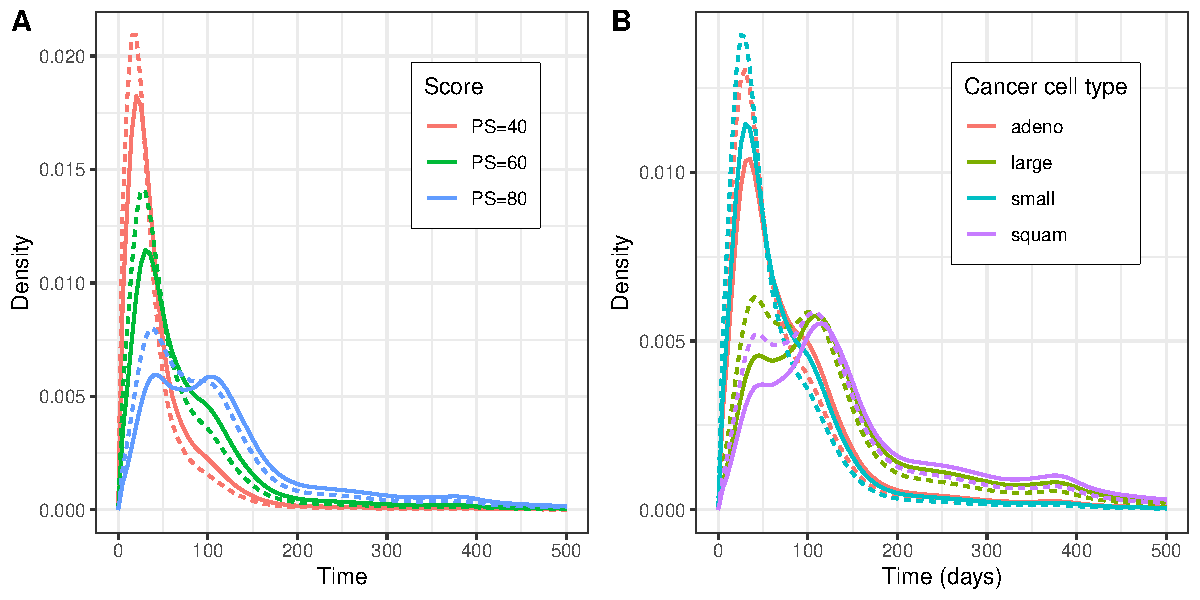
\includegraphics[width=0.8\textwidth]{figs/vet_densities.pdf}\caption{\small Veteran Lung Cancer Trial - Predictive densities of survival time with (dotted) and without (regular) treatment effect. The left panel (A) shows results for $small$ cell type. In the right panel (B), the Karnofsky performance score was fixed at $60$.}\label{fig:VET1}
   \end{figure}
For illustrative purposes, based on the whole dataset, we considered an additional proportional odds (PO) BCTM only including the treatment effect $\big(\varthetavec,F_\text{SL}, (\avec(t)^T, \allowbreak\mathcal{I}(treatment)^T), \pi_{\vartheta}(\varthetavec)\big)$ resulting in the transformation function
\begin{align*}
h(y|\xvec) = \avec(t)^\top \gammavec_1  +\mathcal{I}(treatment)\gamma_2.
\end{align*}
 Here, $\beta$ is the log-odds ratio for the treatment. We can drop the proportional odds assumption by including an interaction term in the model $\big(F_{\text{SL}}, \allowbreak(\avec(t)^\top \otimes (1, \allowbreak\mathcal{I}(treatment)^\top), \allowbreak\pi_{\vartheta}(\varthetavec)\big)$ (NPO) with transformation function
\begin{align*}
h(t| treatment, \xvec) = \avec(t)^\top \gammavec_1 +\mathcal{I}(treatment)\avec(t)^\top\gammavec_2.
\end{align*}
The second term can be interpreted as the deviation from a constant log-odds ratio treatment effect.
The PO model resulted in a WAIC (DIC) of $191.0$ ($191.0$), while the NPO model resulted in a WAIC (DIC) of $192.6$ ($192.2$), indicating that the PO model is preferable in this case. It is straightforward to include nonlinear covariate effects at the cost of more challenging interpretability.
\FloatBarrier


\section{Further Simulation Results}\label{supp:sim}

\begin{table}[H]
    \centering
    \begin{tabular}{l|c}
    \hline\hline
         Model & Specification\\
         \hline 
        Lin. BCTM & $\big( \varthetavec, \Phi,((1,y) \otimes (1,\xvec_p^\top))^\top,\allowbreak \pi_\vartheta(\cdot)\big)$\\
       Lin. MLT & $\big( \varthetavec, \Phi,((1,y) \otimes (1,\xvec_p^\top))^\top \big)$\\
        Full BCTM &  $\big(\varthetavec,\Phi,(\avec_{10}(y)^\top \otimes ( \bvec_{10}(x_1)^\top, \ldots,\allowbreak \bvec_{10}(x_{p+2})^\top))^\top, \pi_\vartheta(\varthetavec)\big)$\\
        Full MLT & $(\avec_{\text{Bs},10}(y)^\top \otimes ( \bvec_{\text{Bs},10}(x_1)^\top, \ldots, \bvec_{\text{Bs},10}(x_{p+2})^\top))^\top$ \\
       Oracle BAMLSS &  $\eta_{\mu} = \beta_0 + x_2 \cdot f_{20}(x_1) + \sum_{k=0}^p f_{20}(x_{2+k})$ and $\eta_{\sigma^2}= \beta_0 + f_{20}(x_1)$  \\
        BAMLSS QR & $\eta_\tau = \sum_{k=0}^{p} f_{2+k,20,\tau}(x_{2+k})$\\
        \hline\hline
    \end{tabular}
    \caption{Simulation study. Model specifications with corresponding basis dimensions in the subscript. Parameter $p$ specifies the number of noise parameters. For the MLT specifications, the basis functions are Bernstein polynomials and for the other models B-splines. The subscripts denote the number of basis functions each.}
    \label{tab:sim:models}
\end{table}

\subsection{Coverage rates}
This section contains results for $n=\{100, 500\}$ and effect estimates from the second simulation setting
Furthermore, empirical coverage rates of pointwise 95\% credible intervals for $n=500$ are shown in Figure \ref{fig:cov2}.


% \begin{figure}[ht]
% 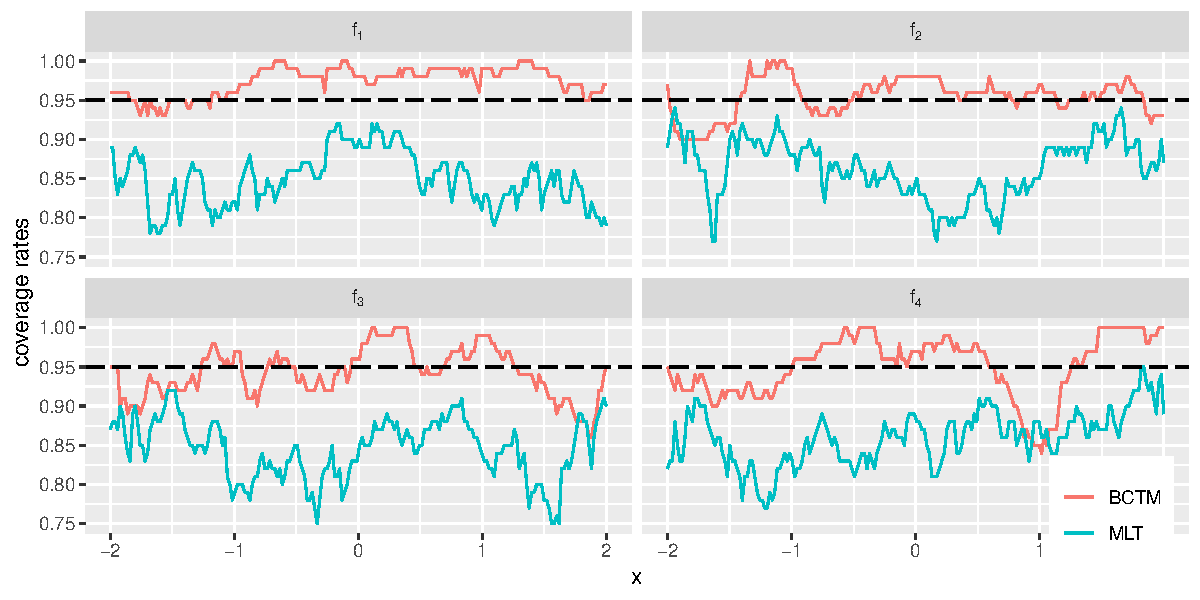
\includegraphics[width=\textwidth]{figs/coverages_n100.pdf}
% \caption{\footnotesize Simulation 2. Coverage rates of pointwise 95\% credible/confidence intervals of BCTM and MLT in each covariate value $x_1, \ldots, x_4$ for $n=100$.}\label{fig:cov1}
% \end{figure}

\begin{figure}
\centering
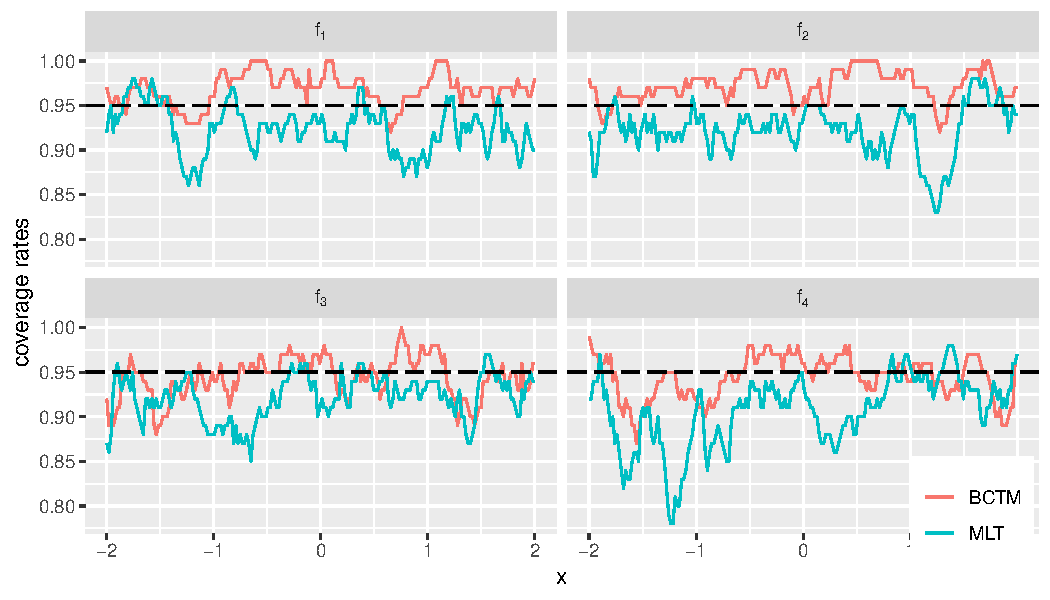
\includegraphics[width=\textwidth]{figs/coverages_n500.pdf}
\caption{\footnotesize Simulation 2. Coverage rates of pointwise 95\% credible/confidence intervals of BCTM and MLT in each covariate value $x_1, \ldots, x_4$ for $n=500$.}\label{fig:cov2}
\end{figure}


\clearpage
\subsection{Effect estimates}
This section shows effect estimates obtained from the BCTM, the MLT and tramME for $n=100$ and $n=500$. Estimation of $f_1(x_1)$ resulted in numerical problems in most replications for tramME.
\begin{figure}[!ht]
\begin{center}
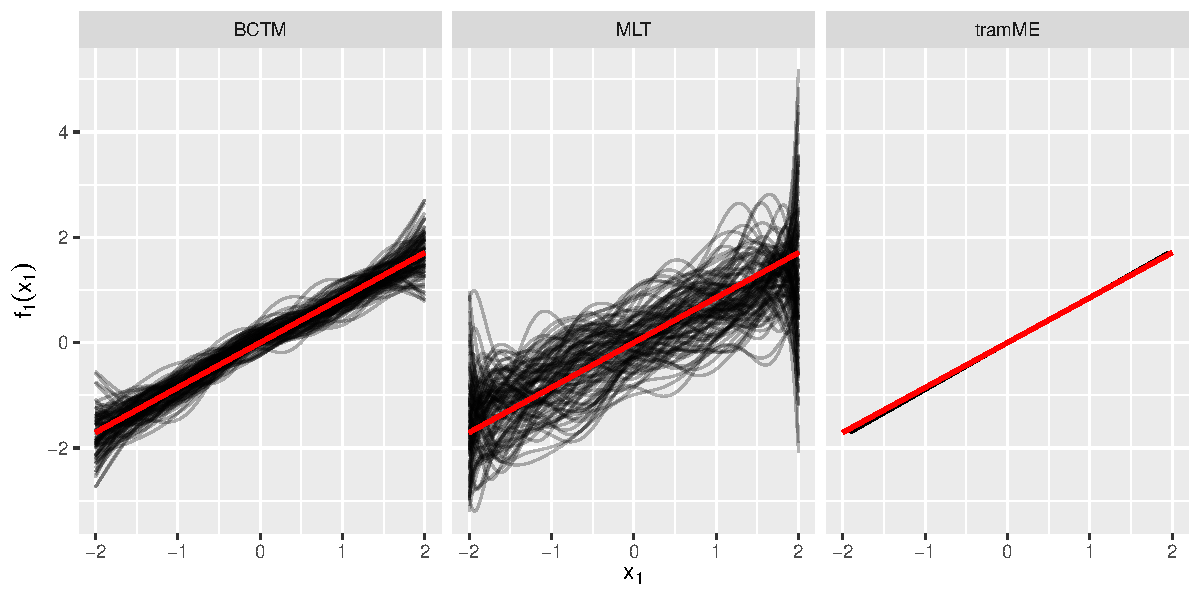
\includegraphics[width=\textwidth]{figs/coverage_f1_n100_wtramme.pdf}
\caption{\footnotesize Simulation 2. $n=100$. Posterior mean estimates of $f_1(x_1)$ of $100$ replications obtained from BCTM and MLT.}\label{fig:eff1_n100}
\end{center}
\end{figure}

\begin{figure}[!ht]
\begin{center}
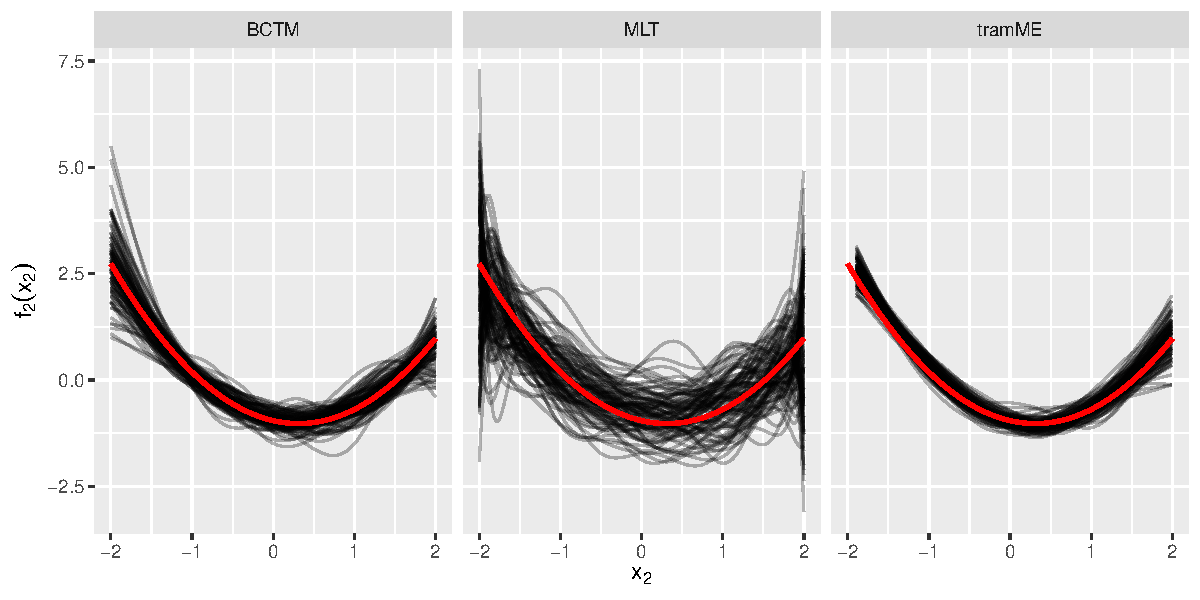
\includegraphics[width=\textwidth]{figs/coverage_f2_n100_wtramme.pdf}
\caption{\footnotesize Simulation 2. $n=100$. Posterior mean estimates of $f_2(x_2)$ of $100$ replications obtained from BCTM and MLT.}\label{fig:eff2_n100}
\end{center}
\end{figure}

\begin{figure}[!ht]
\centering
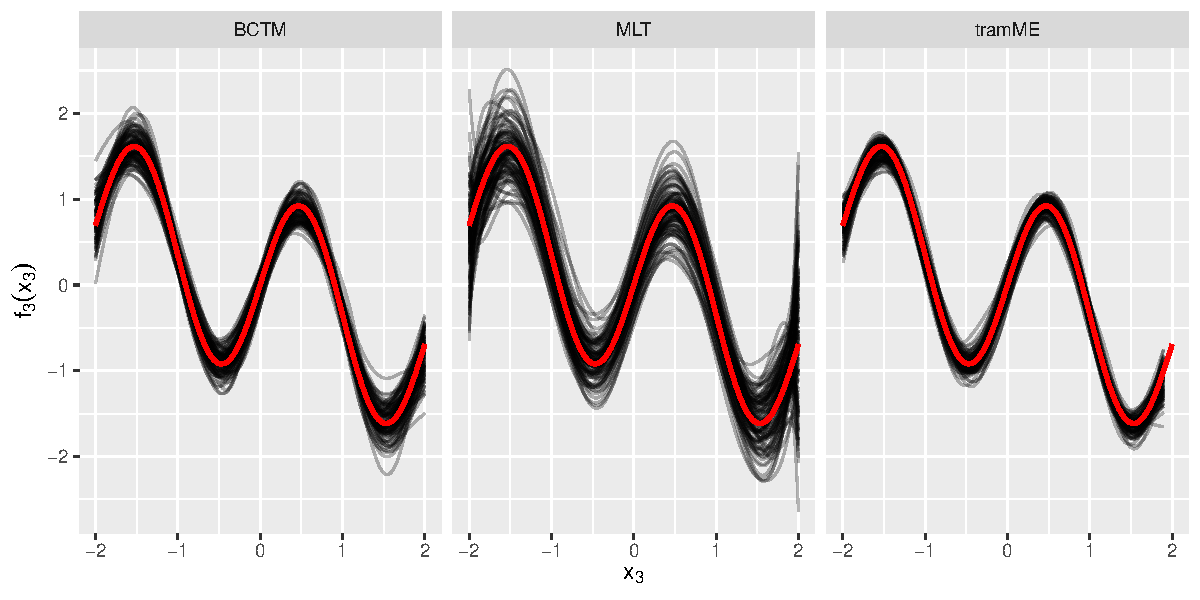
\includegraphics[width=\textwidth]{figs/coverage_f3_n100_wtramme.pdf}
\caption{\footnotesize Simulation 2. $n=100$. Posterior mean estimates of $f_3(x_3)$ of $100$ replications obtained from BCTM and MLT.}\label{fig:eff3_n100}
\end{figure}


\begin{figure}[!ht]
\centering
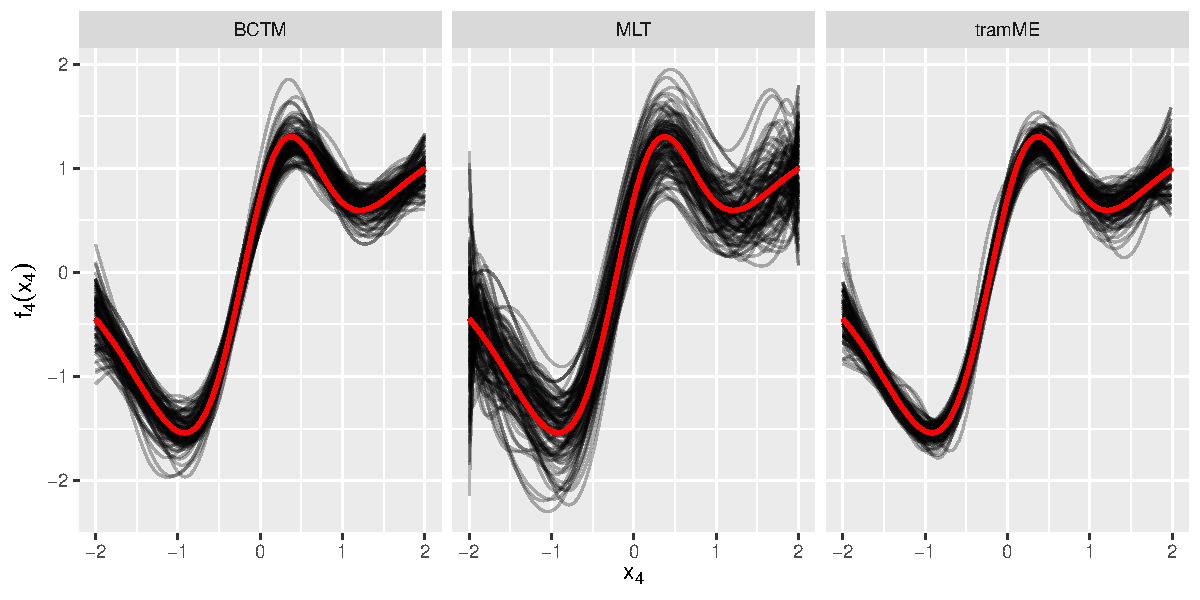
\includegraphics[width=\textwidth]{figs/coverage_f4_n100_wtramme.pdf}
\caption{\footnotesize Simulation 2. $n=100$. Posterior mean estimates of $f_4(x_4)$ of $100$ replications obtained from BCTM and MLT.}\label{fig:eff4_n100}
\end{figure}
%\bibliography{lit}

\begin{figure}[!ht]
\begin{center}
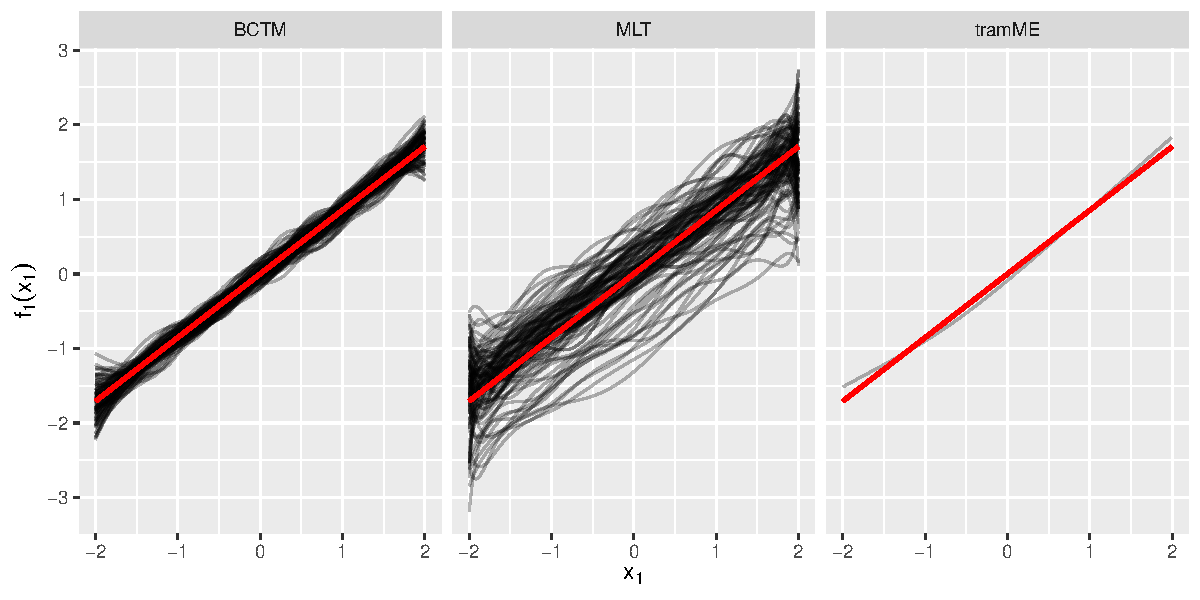
\includegraphics[width=\textwidth]{figs/coverage_f1_n500_wtramme.pdf}
\caption{\footnotesize Simulation 2. $n=500$. Posterior mean estimates of $f_1(x_1)$ of $100$ replications obtained from BCTM and MLT.}\label{fig:eff1_n500}
\end{center}
\end{figure}

\begin{figure}[!ht]
\begin{center}
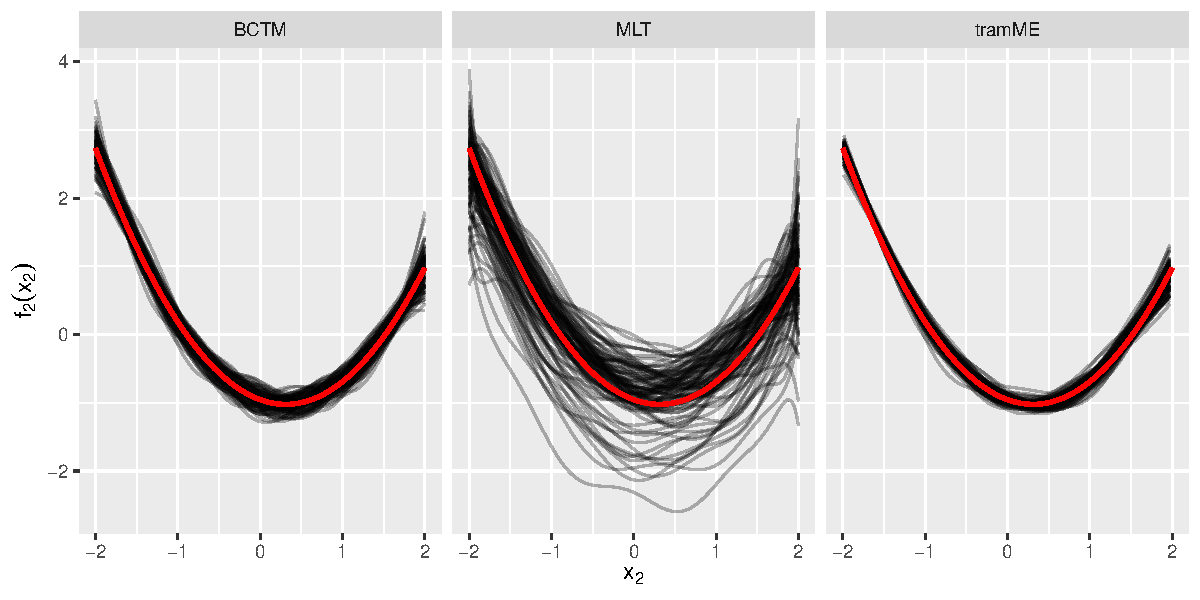
\includegraphics[width=\textwidth]{figs/coverage_f2_n500_wtramme.pdf}
\caption{\footnotesize Simulation 2. $n=500$. Posterior mean estimates of $f_2(x_2)$ of $100$ replications obtained from BCTM and MLT.}\label{fig:eff2_n500}
\end{center}
\end{figure}

\begin{figure}[!ht]
\centering
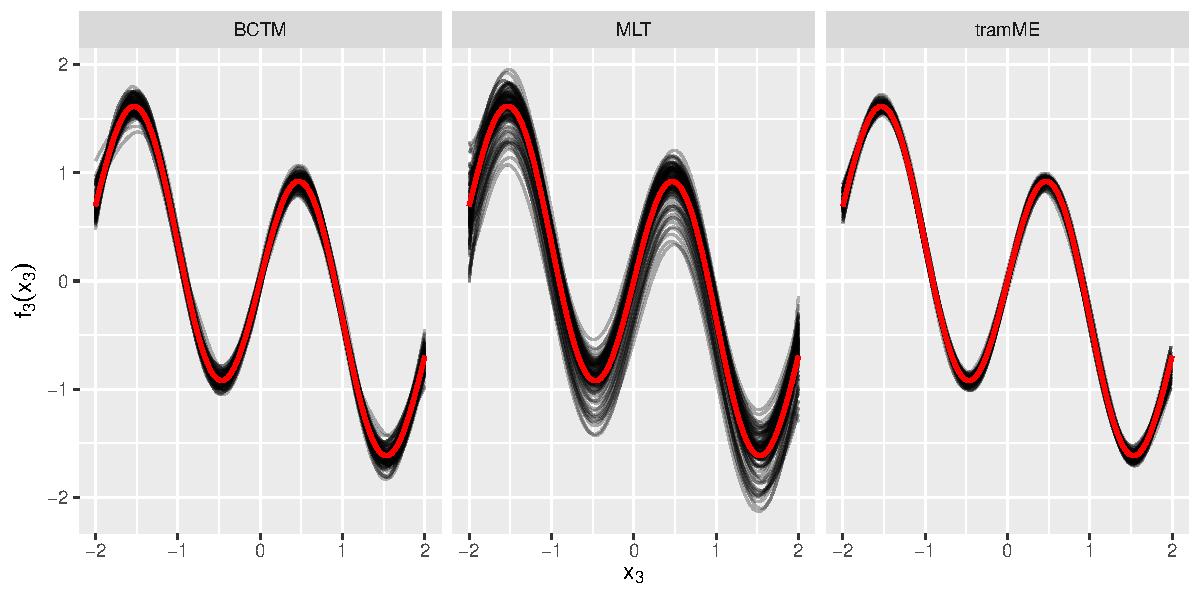
\includegraphics[width=\textwidth]{figs/coverage_f3_n500_wtramme.pdf}
\caption{\footnotesize Simulation 2. $n=500$. Posterior mean estimates of $f_3(x_3)$ of $100$ replications obtained from BCTM and MLT.}\label{fig:eff3_n500}
\end{figure}


\begin{figure}[!ht]
\centering
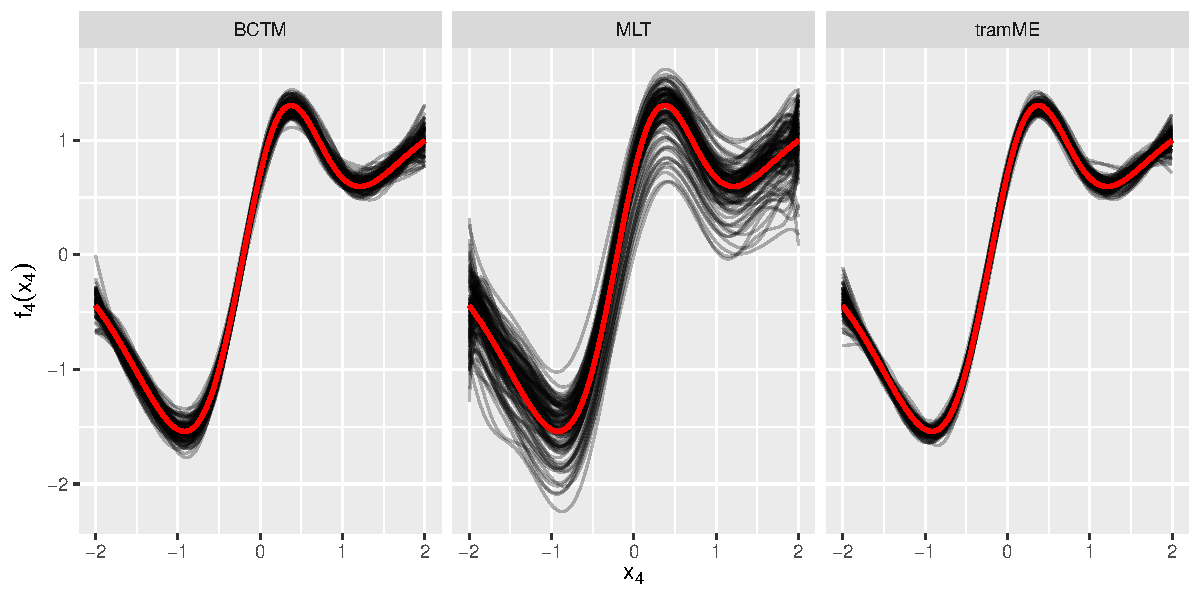
\includegraphics[width=\textwidth]{figs/coverage_f4_n500_wtramme.pdf}
\caption{\footnotesize Simulation 2. $n=500$. Posterior mean estimates of $f_4(x_4)$ of $100$ replications obtained from BCTM and MLT.}\label{fig:eff4_n500}
\end{figure}

\FloatBarrier



\bibliography{lit}


\end{document}

